\documentclass{article}

% if you need to pass options to natbib, use, e.g.:
% \PassOptionsToPackage{numbers, compress}{natbib}
% before loading nips_2016
%
% to avoid loading the natbib package, add option nonatbib
% \usepackage[nonatbib]{nips_2016}

\usepackage{nips_2016}

% to compile a camera-ready version, add the [final] option, e.g.:
%\usepackage[final]{nips_2016}


\usepackage[english, status=draft]{fixme} % these 2 make fixme comments :) 
\fxusetheme{color}                        %

\usepackage[utf8]{inputenc} % allow utf-8 input
\usepackage[T1]{fontenc}    % use 8-bit T1 fonts
\usepackage{hyperref}       % hyperlinks
\usepackage{url}            % simple URL typesetting
\usepackage{booktabs}       % professional-quality tables
\usepackage{amsfonts}       % blackboard math symbols
\usepackage{nicefrac}       % compact symbols for 1/2, etc.
\usepackage{microtype}      % microtypography
\usepackage{graphicx}       %PICTSCHA
\usepackage{amsmath}        %METH, ok appears to be included in the amsfontz





%%%%%%%%%%
% citation stuff
%%%%%%%%

\usepackage{natbib} 
%bibstyle muss einer da sein, 
% setimmt wie der kram an \cite aussieht.
% https://de.wikibooks.org/wiki/LaTeX-W%C3%B6rterbuch:_bibliographystyle
%https://de.sharelatex.com/learn/Bibtex_bibliography_styles
%\bibliographystyle{abbrvnat} 
\bibliographystyle{unsrt} 
%\bibliographystyle{plainnat}









\title{A constructive approach for graphs\\with long range dependencies}

% The \author macro works with any number of authors. There are two
% commands used to separate the names and addresses of multiple
% authors: \And and \AND.
%
% Using \And between authors leaves it to LaTeX to determine where to
% break the lines. Using \AND forces a line break at that point. So,
% if LaTeX puts 3 of 4 authors names on the first line, and the last
% on the second line, try using \AND instead of \And before the third
% author name.

\author{
  Stefan Mautner\\
  Department of Computer Science\\
  Albert-Ludwigs University Freiburg\\
  Freiburg, 79085  \\
  \texttt{mautner@cs.uni-freiburg.de} \\
  %% examples of more authors
  \And
  Fabrizio Costa \\
  Department of Computer Science\\
  Albert-Ludwigs University Freiburg\\
  Freiburg, 79085  \\
  \texttt{costa@informatik.uni-freiburg.de} \\
  %%\AND
  %% Coauthor \\
  %% Affiliation \\
  %% Address \\
  %% \texttt{email} \\
  %% \And
  %% Coauthor \\
  %% Affiliation \\
  %% Address \\
  %% \texttt{email} \\
  %% \And
  %% Coauthor \\
  %% Affiliation \\
  %% Address \\
  %% \texttt{email} \\
}

\begin{document}
% \nipsfinalcopy is no longer used

\maketitle

\begin{abstract}
%Scripts describing the generation of generic graphs based on examples
%are scarce.

Machine learning constructive approaches offer a way to answer interesting
'design' questions on the basis of a collection of examples. Rather than
focusing on the prediction of specific qualities for a given input object,
these methods learn how to synthesize novel instances that share the same
characteristics of a selected sample. In particular, graph constructive
methods are of interest in chemo- and bio-informatics domains where the task
is to synthesize novel molecules with a desired bioactivity. Unfortunately
most molecules exhibit complex dependencies between their different
constituent parts. RNA polymers for example self interact, with nucleotides
forming bounds that can typically span the entire length of the sequence.
Modeling in an efficient way long range dependencies is a particularly
difficult problem. Here we propose a solution, based on graph contractions,
that builds on top of a recent constructive approach and we show encouraging
results on a RNA sequence synthesis task.

% Graphs are flexible data structures whose generation 
% is a mostly unexplored problem. As discriminative systems for graphs
% exist, it is feasible to direct a generative process.
% An existing method is implementing Markov Chain Monte Carlo 
% sampling which is altering graphs incrementally.
% Alteration is done with a \emph{graph grammar}, a collection
% of sub graphs, grouped by exchangeability.

% \fxwarning{so the abstract was rewritten, i made sure to explain the contraction}
% By contracting edges in a graph i.e. merging adjacent vertices,
% we obtain a more abstract view on a graph. 
% We use this abstraction to overcome the shortcomings of the original 
% grammar.
% However, the modification is required to be automatically generate. 
% We explore the application of this idea
% on graphs representing RNA secondary structure. 




\end{abstract}
\section{Introduction}


% 
\begin{figure}[ht]
      \centering
        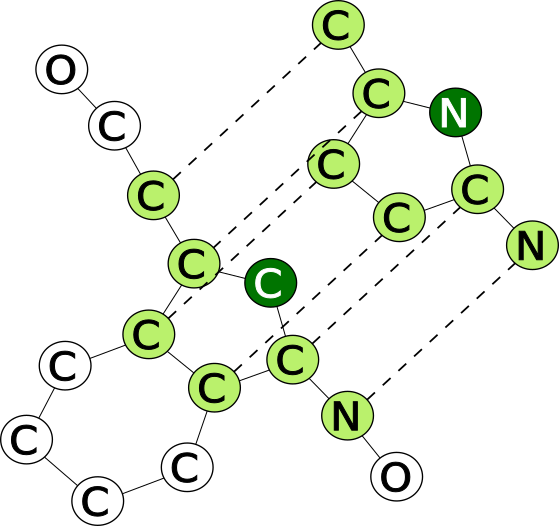
\includegraphics[width=0.2\linewidth]{images/showcip.png}
      \caption{Sample figure caption.}
      \label{nazis}
\end{figure}

\section{Method}
Previously Costa \cite{costa14} introduced a method
to construct novel graphs according to a distribution, which is given by
examples. Graphs are vectorized by a \emph{decomposition kernel}
to train a machine learning model, e.g. an SVM.
Fragments of the graphs are collected in 
a \emph{grammar} (analogous to a string grammar) to alter the initial
set of graphs incrementally. Such changes to a graph are evaluated with the
model. 
We present a method to increase the flexibility of the graph grammar.

\subsection{Previous grammar and definitions}

The grammar consists of sets of interchangeable graph fragments.
We call these fragments core interface pairs(CIPs) because 
they consist of a core part and an interface part.
In terms of a string grammar core and interface are imaginable 
as a production: $iiiCCCiii <-> iiiCCCCiii$. 

If two interfaces are isomorphic, we can exchange the core parts


\subsection{Contribution}
\textbf{Modification to the grammar.}
In place of simple CIPs as used previously,
we use modified CIPs that consider contracted versions
of the original graphs. We obtain a contracted graph $G'$ by contracting edges
in $G$. The set of contracted vertices of a
created vertex is accessible with the $contracted$ function.
The functions for extracting core and interface graphs, 
$C_{R}^v(G')$ and $I_{R,T}^v(G')$, are unaltered except that we apply them
on $G'$ instead of $G$. 
The core graph $C_{R}^v(G',G)$ is induced by the nodes 
$\bigcup\limits_{u \in C_R^v(G')} contracted(u)$.
The new interface graph $I_{R,B}^v(G',G)$ is then obtained by the nodes 
$\{ w | d(w,v) \leq B \wedge v\in C_R^v(G',G) \wedge w \in G \wedge w 
\notin C_R^v(G',G) \}$.  $B$ is the thickness of the base graph. 
\fxwarning{say these formulas first in words}
At this point we can construct a CIP from $C_R^v(G',G)$ and $I_{R,B}^v(G',G)$. 
To find a congruent CIP, we previously compared the hashed $I_{R,T}^v(G)$ 
graphs. By hashing the hashes of $I_{R,T}^v(G')$ and $I_{R,B}^v(G,G')$ we 
increase the specificity of this comparison. The vertices in $I_{R,B}^v(G,G')$ 
might have been relabeled to represent a concept of its $contracted$ set. In 
\fxwarning{usage of CONCEPT  >:(}
our application case, we will contract according to the 
secondary RNA structure and label the resulting vertex accordingly e.g.
'Hairpin loop'. This way we encode far reaching and abstract 
\fxwarning{explain more the ENCODE part}
information about the surrounding vertices in our CIP interface matching.


% graph contration, interface trick
% change to congruency
\textbf{An improvement to the notion of congruency.}
CIPs require isomorphism to be considered congruent.
We expand this requirement to incorporate
the distance to the closest nodes in the core graph when 
determining if graphs are congruent.
$\forall u \in I_{R,T}^v(G) : 
\underset{z \in  C_{R}^v(G)}{\min} d(u,z) = 
\underset{z' \in  C_{R}^{v'}(G')}{\min} d(\phi(u),z') $ i.e. the distance 
to the closest core node is equal for every
$u$ and $\phi(u)$.
It is easy to see the benefit of this extension.
\fxwarning{ a and b example sounds to casual i think}
imagine two vertices labeled 'a' and 'b' connected by an edge. Let this graph
be the sole interface graph. With the new model we can distinguish 
between 'a' being closer to the core and 'b' being closer. 

\textbf{Extending what we can contract.}
\fxwarning{all of this is questionable. describe problem with unconnected 
nodes, mv rest to eval }
Edge contraction is one way to obtain a contraction graph. 
One might also contract nodes that are not connected by an edge.
We did so with multi-loop nodes except stem nucleotides.
This contraction model however will raise the problem 
of two adjacent stems connected to a multi-loop being
indistinguishable from one stem being connected.
this may be resolved by adding an additional 'fake' vertex 
between the stems. another problem with 
this case is, that the order of the stems would normally get lost.
Since the graph representing the molecule, is directed via 
the backbone one is able to specify an order on the
parts of loops that connect stems.

\fxwarning{remove this eden part.. what about the directedness? look up what 
i did!also the hashing part! and then explain it}
Although the underlying EDeN kernel does not support directed graphs,
the grammar may contain directed graphs. This is implemented by extracting
CIPs as if undirected and creating the grammar as usual.
% need to be able to recalculate abstractions
A constraint to the contraction is that we need to be able to 
generate it algorithmically. In the sampling phase we recalculate 
the contraction after changes to the underlying graph.


\section{Evaluation}
% Infernal is the way to go
\fxwarning{explain the secondary structure}
RNA sequences are sequences over the four nucleotides A,G,U and C.
They have a 5' and a 3' end, meaning that the direction matters.
Nucleotides in the sequences bind to other nucleotides so
the sequence forms a \emph{structure}.
RNAs are grouped into functional families whose classification
is a problem of biology. \emph{Infernal}\cite{infernal} can classify and 
create members of these families using covariance models.
Infernal gives us a domain specific way to evaluate
our Method for the generation of new graphs. 

% choose data this way
We chose our RNA sequences from the seed sequences of each family
that Infernal is using\cite{rfam}. Sequences were chosen from RNA families with
a) many members, because some families contain 10
instances which is very few for a classification task. b) interesting 
structure, many sequences fold into structures that exhibit a large number of 
unpaired bases which would result in a very simple contracted graph
c) similar length, because classification should no be trivial.

% this is how we prepare the graphs
We evaluated our results on secondary RNA structure graphs, were each 
nucleotide is a vertex. The contracted graphs are obtained by 
contracting vertices that belong to the same structural element,
e.g. adjacent stem vertices are contracted into a single vertex.
Secondary structures are obtained by \emph{muscle}-aligning \cite{muscle} with 
\fxwarning{"muscle-aligning" is terrible. explain why we are doing it this way }
the four closest neighbors by sequence and folding with \emph{RNAalifold}
\cite{rnaalifold}.  For RNA sequences, the direction in which a sequence
is read is important.  Working with directed graphs in the grammar
will enable us to extract the sequence along the backbone easily as well
as adapt the model to the directed biological reality.

% eval against Infernal
We evaluate our generated sequences against the Infernal model.
The Infernal model is hand curated and thus highly reliable.
 \textbf{INFERNALEVAL} shows the average bit-score of generated graphs
and the size of the training set. Each family has its own quality threshold.
Sequences above that threshold (marked in black) can reliably be considered
part of the family. We observe that \textbf{y out of x} generated graphs.

% eval learning curve+ edit dist
Costa \cite{costa14} defines \emph{the constructive learning problem for 
finite samples} 
as mimicking the distribution of given graphs while producing new instances.
We can estimate this distribution with a machine learning
model and compare two distributions by evaluating a set of test instances
on the models. We can also measure how different generated sequences
are by comparing the edit distance.
\textbf{SOMEGRAPHZ} shows the learning curves for the original set
of graphs and the generated set. Notice, that they are very similar.
We can also see the average edit distance for the generated graphs 
to their closest match in the original set.

% eval vs classical method
The method presented here is adapting an older method to new problems.
\textbf{SOMEGRAPHZ} is a repetition of the first experiment with 
the old algorithm. We observe that its not producing reliable
graphs.
\begin{figure}[ht]
      \centering
        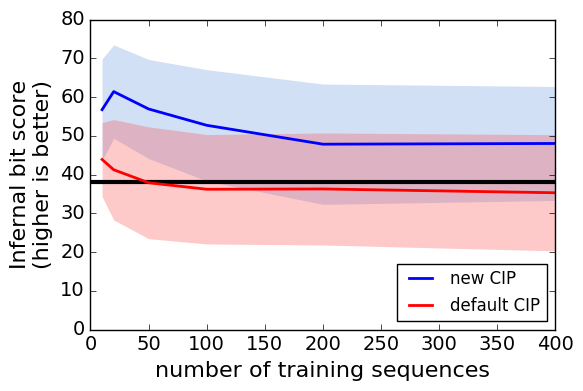
\includegraphics[width=0.8\linewidth]{images/infernal_abstr.png}
      \caption{Infernal evaluation on new method}
      \label{nazis}
\end{figure}
\fxwarning{ should we merge the 2 infernal charts?}
\fxwarning{pictures are not in their final form}
\begin{figure}[ht]
      \centering
        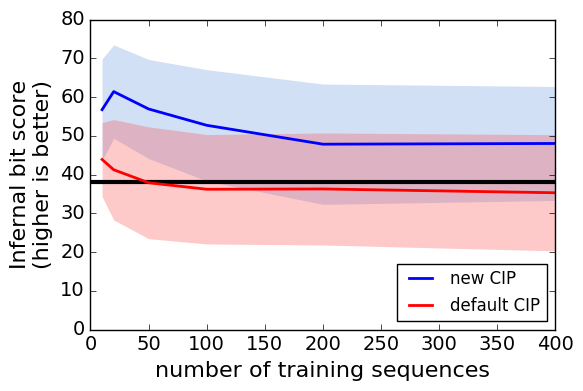
\includegraphics[width=0.8\linewidth]{images/infernal_abstr.png}
      \caption{infernal on unabstract graphlearn}
      \label{nazis}
\end{figure}
\begin{figure}[ht]
      \centering
        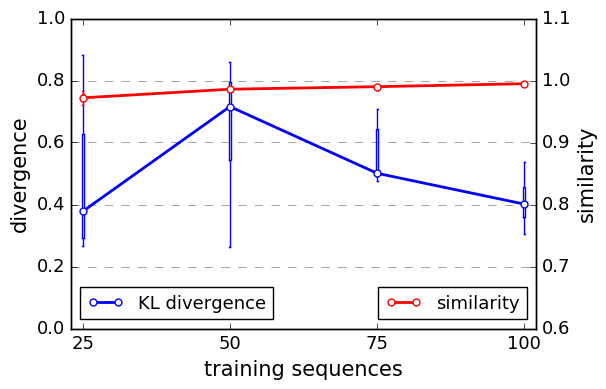
\includegraphics[width=0.8\linewidth]{images/learningcurve.png}
      \caption{learning curve}
      \label{nazis}
\end{figure}



\section{Discussion} 
We have compared the algorithm to its predecessor and shown
that its result hold up in a state of the art, domain specific
evaluation. Its drawback is the reliance on the ability to 
generate a contraction. In some domains this contraction is 
obvious as in chemical compounds cycles or charge maps are good candidates.
For the general case the contraction can be learned.

\fxwarning{general things: add pictures}
\bibliography{mybib}


\end{document}

